\documentclass[sigconf]{acmart}

\AtBeginDocument{%
  \providecommand\BibTeX{{%
    \normalfont B\kern-0.5em{\scshape i\kern-0.25em b}\kern-0.8em\TeX}}}

\usepackage{dblfloatfix}
\usepackage{mathtools}
\usepackage{hyperref}
\usepackage[htt]{hyphenat}
\usepackage{listings}
\usepackage{xcolor}
\usepackage[framemethod=tikz]{mdframed}
\usepackage{tikz}
\usetikzlibrary{shapes,arrows}

\definecolor{codegreen}{rgb}{0,0.6,0}
\definecolor{codegray}{rgb}{0.5,0.5,0.5}
\definecolor{codepurple}{rgb}{0.58,0,0.82}
\definecolor{backcolour}{rgb}{0.95,0.95,0.92}

\lstdefinestyle{mystyle}{
	backgroundcolor=\color{backcolour},
	commentstyle=\color{codegreen},
	keywordstyle=\color{magenta},
	numberstyle=\tiny\color{codegray},
	stringstyle=\color{codepurple},
	basicstyle=\ttfamily\footnotesize,
	breakatwhitespace=false,
	breaklines=true,
	captionpos=b,
	keepspaces=true,
	numbers=left,
	numbersep=5pt,
	showspaces=false,
	showstringspaces=false,
	showtabs=false,
	tabsize=2,
}

\lstset{style=mystyle}

\begin{document}

\title{Enhancement of images with uneven illumination}
\subtitle{Enhancing images with uneven illumination using ensemble learning\\Group ID: \#1}

% AUTHORS:
\author{Til Mohr}
\affiliation{}
\email{tv.mohr@stud.uis.no}

\author{Alexander Mühleisen}
\affiliation{}
\email{???}

% DATE:
\date{\today}



\begin{abstract}

\end{abstract}

\keywords{image processing, image enhancement, uneven illumination, ensemble learning}

%% Remove copyright footer
\settopmatter{printacmref=false}
\setcopyright{none}
\renewcommand\footnotetextcopyrightpermission[1]{}
\pagestyle{plain}
%% ------------------------

%%
%% This command processes the author and affiliation and title
%% information and builds the first part of the formatted document.
\maketitle


\section{Introduction}\label{sec:intro}

\section{Theory}\label{sec:theory}
In this section we will dive into different methods to enhance images with uneven illumination. We will start with a brief introduction to the problem and then discuss different methods to solve it. We will also discuss the advantages and disadvantages of each method, and from this conclude particular use cases where they might be helpful.

\subsection{Problem description}\label{sec:problem}
Uneven illumination refers to the irregular distribution of light intensity across an image. In essence, it disrupts the uniformity of the visual output, leading to disparities in brightness and contrast, often observable as glares or shadows. These disparities can mask essential features and details, making the subject of the image less identifiable. This becomes especially problematic when images need to be processed further for various computer vision tasks. In fields like optical microscopy, for example, consistent illumination is crucial for accurately identifying and segmenting microscopic entities. Uneven lighting can obscure crucial cellular structures or make similar-looking entities appear distinct, hampering accurate analysis \cite{dey2019uneven}.

To counter this issue, the goal is to enhance the image in a manner that simulates its capture under uniform illumination conditions. By doing so, we aim to restore a natural appearance to the image, preserving details and minimizing artifacts introduced by uneven lighting. This correction enables better analysis, ensuring that conclusions drawn are based on the actual subject and not on lighting imperfections \cite{dey2019uneven}.

\subsection{Unsharp Masking}\label{sec:unsharp}

\subsection{Retinex}\label{sec:retinex}

\subsection{Homomorphic Filtering}\label{sec:homomorphic}
The intensity of an image at pixel $(x,y)$ can be described as the product of the illumination $i(x,y)$ and the reflectance $r(x,y)$ \cite{voicu1997practical,fan2011homomorphic}:
\begin{equation}
	f(x,y) = i(x,y) \cdot r(x,y)
\end{equation}
In the frequency domain, illumination changes across the image are typically manifested by low frequencies, while high frequencies are associated with reflectance changes. Therefore, by applying the logarithm to the image, one can separate the illumination and reflectance components of the image \cite{voicu1997practical,fan2011homomorphic}:
\begin{equation}
	\log(f(x,y)) = \log(i(x,y)) + \log(r(x,y))
\end{equation}
Applying the Fourier transform to this log-image, a filter $H(u,v)$ can be applied to attenuate the low frequencies, that is the frequencies responsible for illumination changes, and increasing the high frequencies responsible for detail. Afterwards, by applying the inverse Fourier transform and the exponential function, the image can be enhanced \cite{voicu1997practical,fan2011homomorphic}:
\begin{equation}
	f(x,y) = \exp(\mathcal{F}^{-1}(\mathcal{F}(\log(f(x,y))) \cdot H(u,v)))
\end{equation}
This process is illustrated in Figure \ref{fig:homomorphic-pipeline}.

\begin{figure}
	\centering
	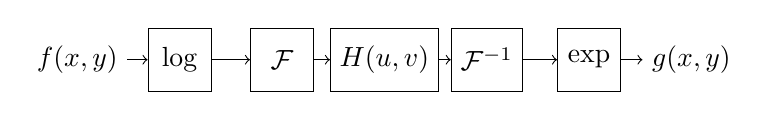
\begin{tikzpicture}[node distance=1.3cm, auto]
		% Define the style for the operation nodes
		\tikzstyle{operation}=[rectangle, draw=black, minimum size=0.8cm, text centered]

		% Define nodes
		\node (input) {$f(x,y)$};
		\node (op1) [operation, right of=input] {$\log$};
		\node (op2) [operation, right of=op1] {$\mathcal{F}$};
		\node (op3) [operation, right of=op2] {$H(u,v)$};
		\node (op4) [operation, right of=op3] {$\mathcal{F}^{-1}$};
		\node (op5) [operation, right of=op4] {$\exp$};
		\node (output) [right of=op5] {$g(x,y)$};

		% Define edges
		\draw[->] (input) -- (op1);
		\draw[->] (op1) -- (op2);
		\draw[->] (op2) -- (op3);
		\draw[->] (op3) -- (op4);
		\draw[->] (op4) -- (op5);
		\draw[->] (op5) -- (output);
	\end{tikzpicture}
	\caption{Homomorphic filtering pipeline.}
	\label{fig:homomorphic-pipeline}
\end{figure}

Many approaches to the linear filter $H(u,v)$ exist. Voicu et al. propose to use a second order Butterworth filter \cite{voicu1997practical}, to reduce the low frequencies and enhance the high frequencies:
\begin{align}
	H(u, v) = H'(\rho) = \gamma_1  - \gamma_2 \cdot \frac{1}{1 + 2.415 \cdot \left(\frac{\rho}{\rho_c}\right)^{4}},\\
	\text{where} \qquad \rho = \sqrt{u^2 + v^2}
\end{align}
where $\gamma_1, \gamma_2, \rho_c$ are parameters that can be tuned to achieve the desired effect. The resulting filter has the general form shown in Figure \ref{fig:homomorphic-filter} \cite{voicu1997practical}.

\begin{figure}
	\centering
	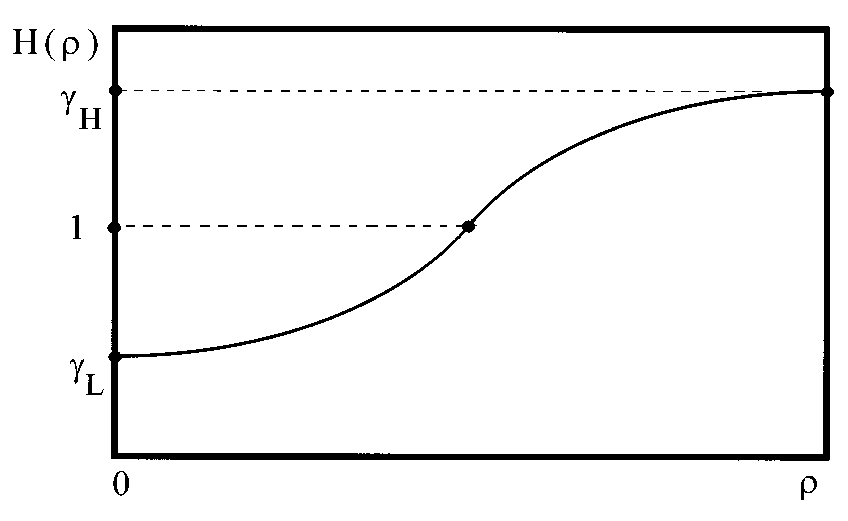
\includegraphics[width=0.45\textwidth]{images/filter.png}
	\caption{General form of the filter used in homomorphic filtering \cite{voicu1997practical}.}
	\label{fig:homomorphic-filter}
\end{figure}

Finally, Fan et al. \cite{fan2011homomorphic} propose  to append a histogram equalization step to the homomorphic filtering pipeline, in order to improve the contrast of the image. An implementation of this approach is shown in Listing \ref{lst:homomorphic}.


\section{Methodology}\label{sec:method}

\section{Results}\label{sec:results}


\section{Discussion and Conclusions}


%%
%% If your work has an appendix, this is the place to put it.
\appendix

\section{Listings}
\subsection{Homomorphic Filtering}\label{sec:homomorphic-listing}
\begin{mdframed}[backgroundcolor=backcolour,leftmargin=0cm,hidealllines=true,innerleftmargin=0cm,innerrightmargin=0cm,innertopmargin=0cm,innerbottommargin=-0.65cm]
\lstinputlisting[language=Python, caption=Homomorphic filtering, label=lst:homomorphic]{listings/homomorphic_filtering.py}
\end{mdframed}


%%
%% The next two lines define the bibliography style to be used, and
%% the bibliography file.
\bibliographystyle{ACM-Reference-Format}
\bibliography{main}

\newpage
\appendix

\end{document}
\endinput
